\documentclass[aspectratio=169,11pt]{beamer}

\usetheme{Madrid}
\usecolortheme{default}
\usefonttheme{professionalfonts}
\setbeamertemplate{navigation symbols}{}
\setbeamertemplate{footline}[frame number]

\usepackage{amsmath, amssymb, booktabs, graphicx}
\graphicspath{{../../assets/figures/}{assets/figures/}}

\title{Monopsony, Measurement, and Sources of Power}
\subtitle{Labor II --- Week 6}
\author{Teaching deck draft}
\date{}

\begin{document}

\begin{frame}
  \titlepage
\end{frame}

\begin{frame}{Central question and course repositioning}
\begin{itemize}
    \item What does it mean to say that firms have wage-setting power in labor markets?
    \item Week 6 turns Week 5's wage-setting protocols into measurable labor market power.
    \item Week 7 will then ask how policy works once firms face finite labor supply to the firm.
\end{itemize}
\end{frame}

\begin{frame}{Week 5 to Week 6 bridge}
\begin{itemize}
    \item Week 5: posting, bargaining, and internal pay rules tell us how wages are set.
    \item Week 6: monopsony tells us how much power employers have inside those protocols.
    \item The new empirical objects are labor supply to the firm, markdowns, concentration, mergers, and pass-through.
\end{itemize}
\end{frame}

\begin{frame}{Course map}
\begin{center}
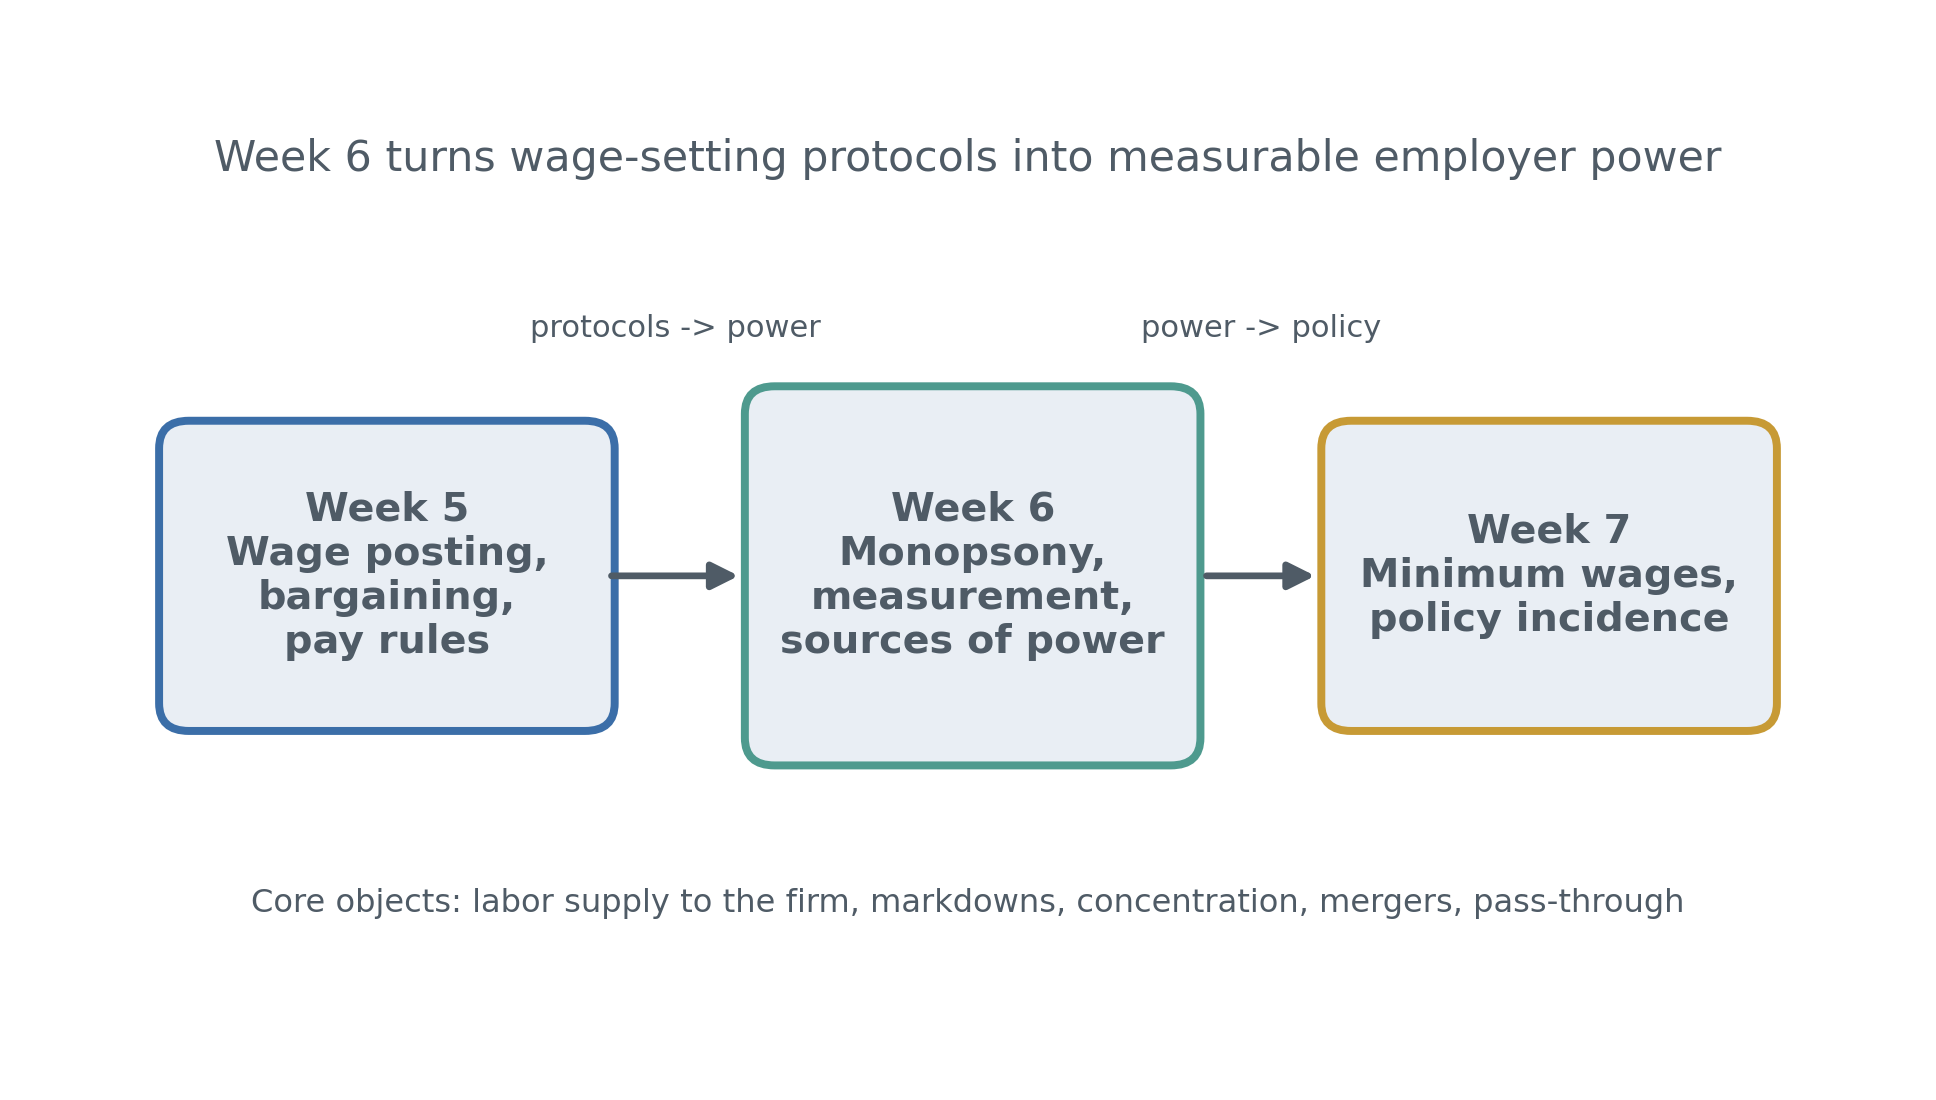
\includegraphics[width=0.84\linewidth]{06-monopsony-course-map.png}
\end{center}
\end{frame}

\begin{frame}{What monopsony is and is not}
\begin{itemize}
    \item Monopsony is employer wage-setting power, not only the literal one-employer town.
    \item The firm faces upward-sloping labor supply to the firm rather than perfectly elastic labor supply.
    \item Concentration, employer size, and labor market power are related but not identical objects.
\end{itemize}
\end{frame}

\begin{frame}{Classic monopsony versus modern dynamic/search monopsony}
\begin{center}
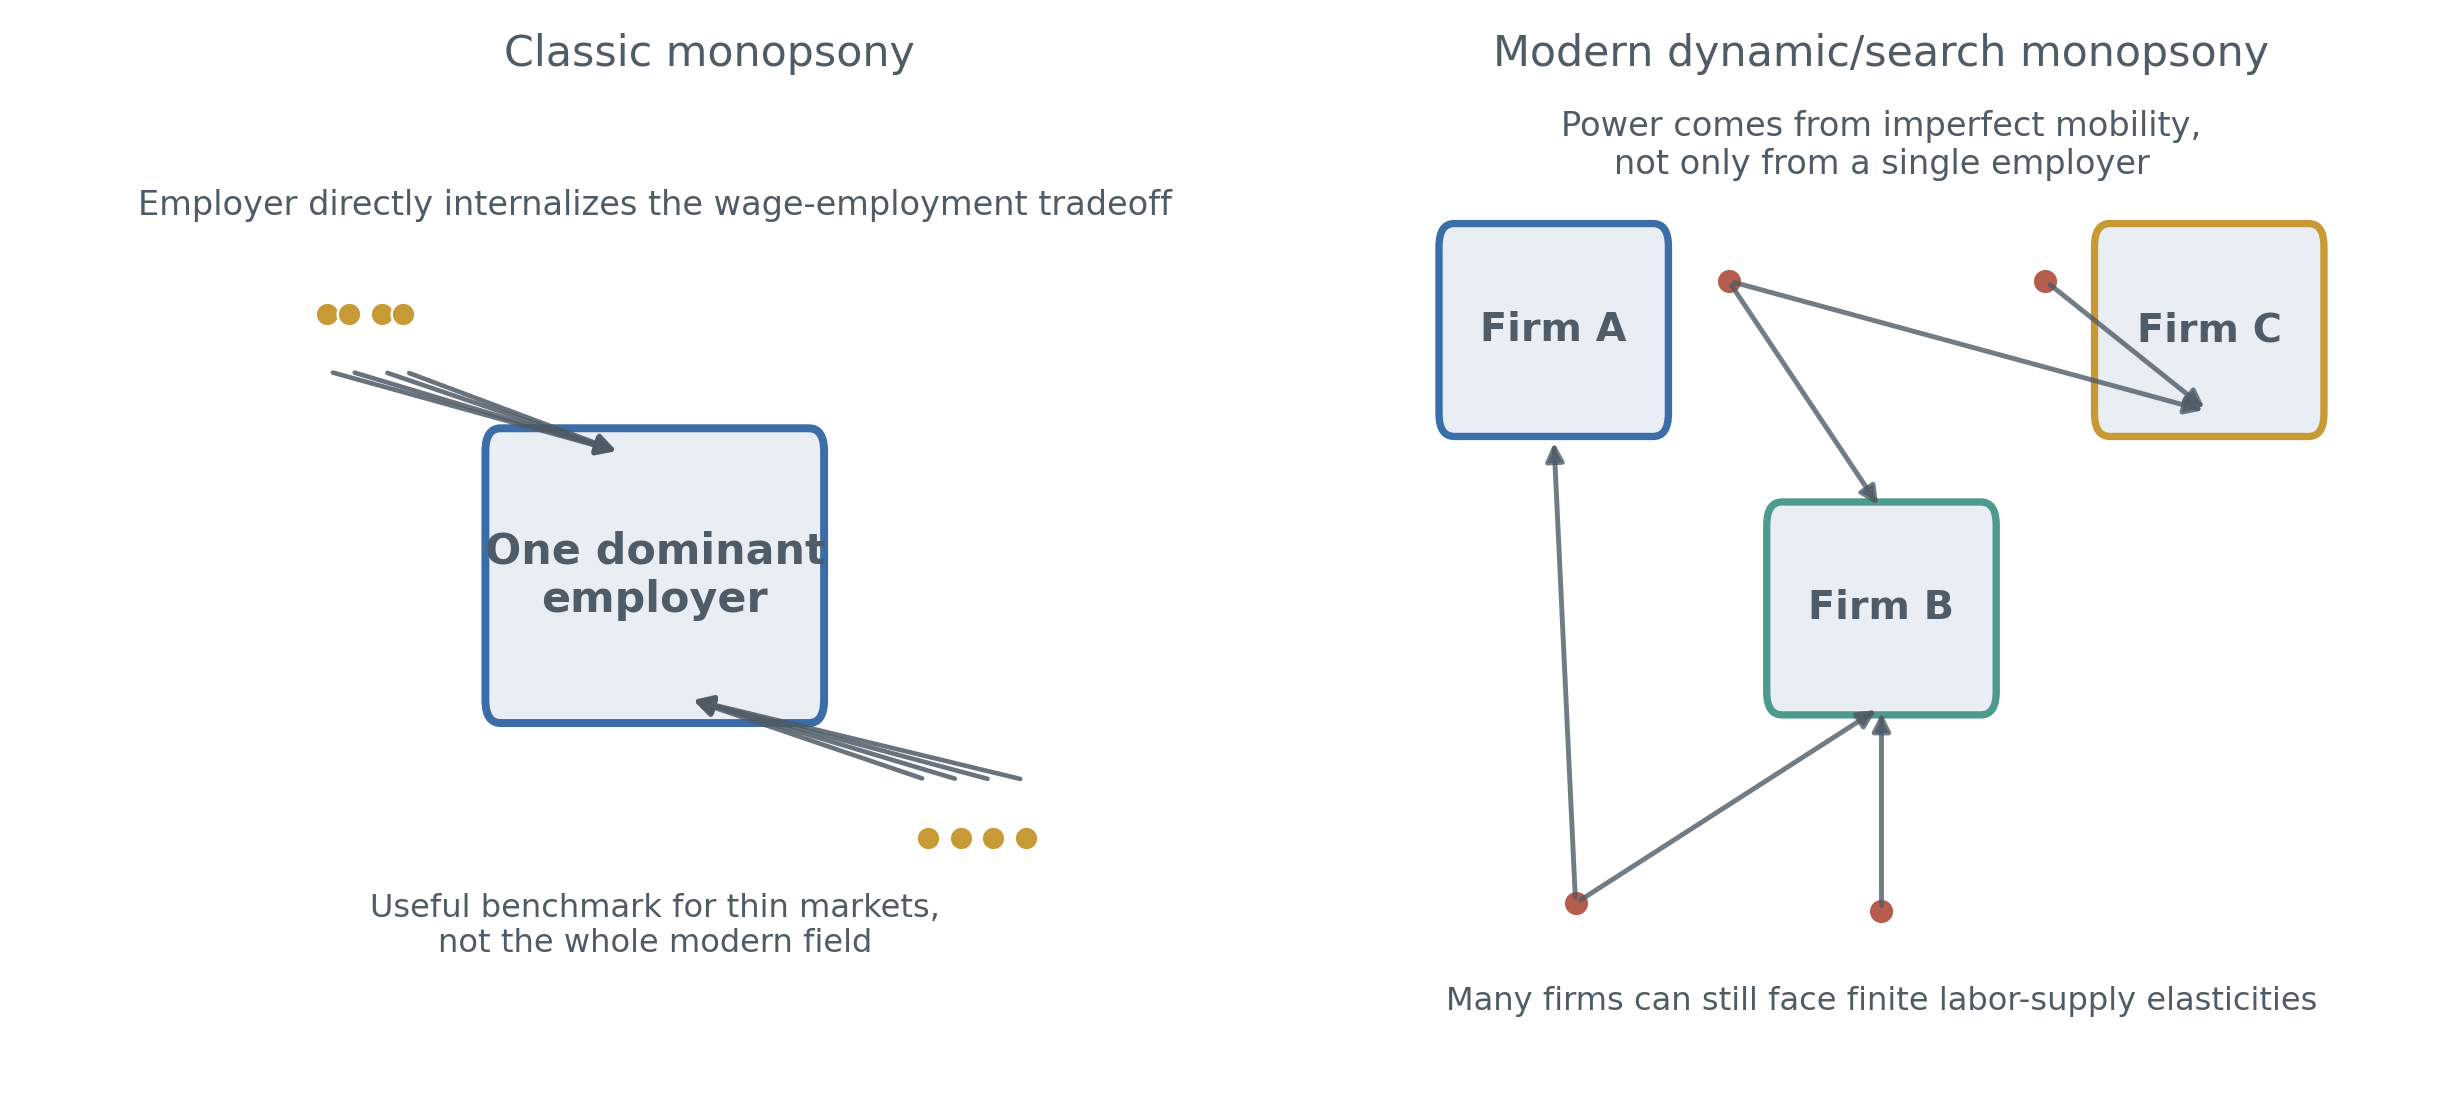
\includegraphics[height=0.72\textheight]{06-classic-vs-modern-monopsony.png}
\end{center}
\end{frame}

\begin{frame}{Labor supply to the firm}
\[
\varepsilon_{N,w}
=
\frac{\partial \log N(w)}{\partial \log w}
\]

\begin{itemize}
    \item The relevant elasticity is employment at a firm with respect to that firm's own wage.
    \item This is not the same object as market labor supply.
    \item Modern monopsony can exist even with many firms if worker mobility is imperfect.
\end{itemize}
\end{frame}

\begin{frame}{Labor supply, wage-setting power, and marginal labor cost}
\begin{center}
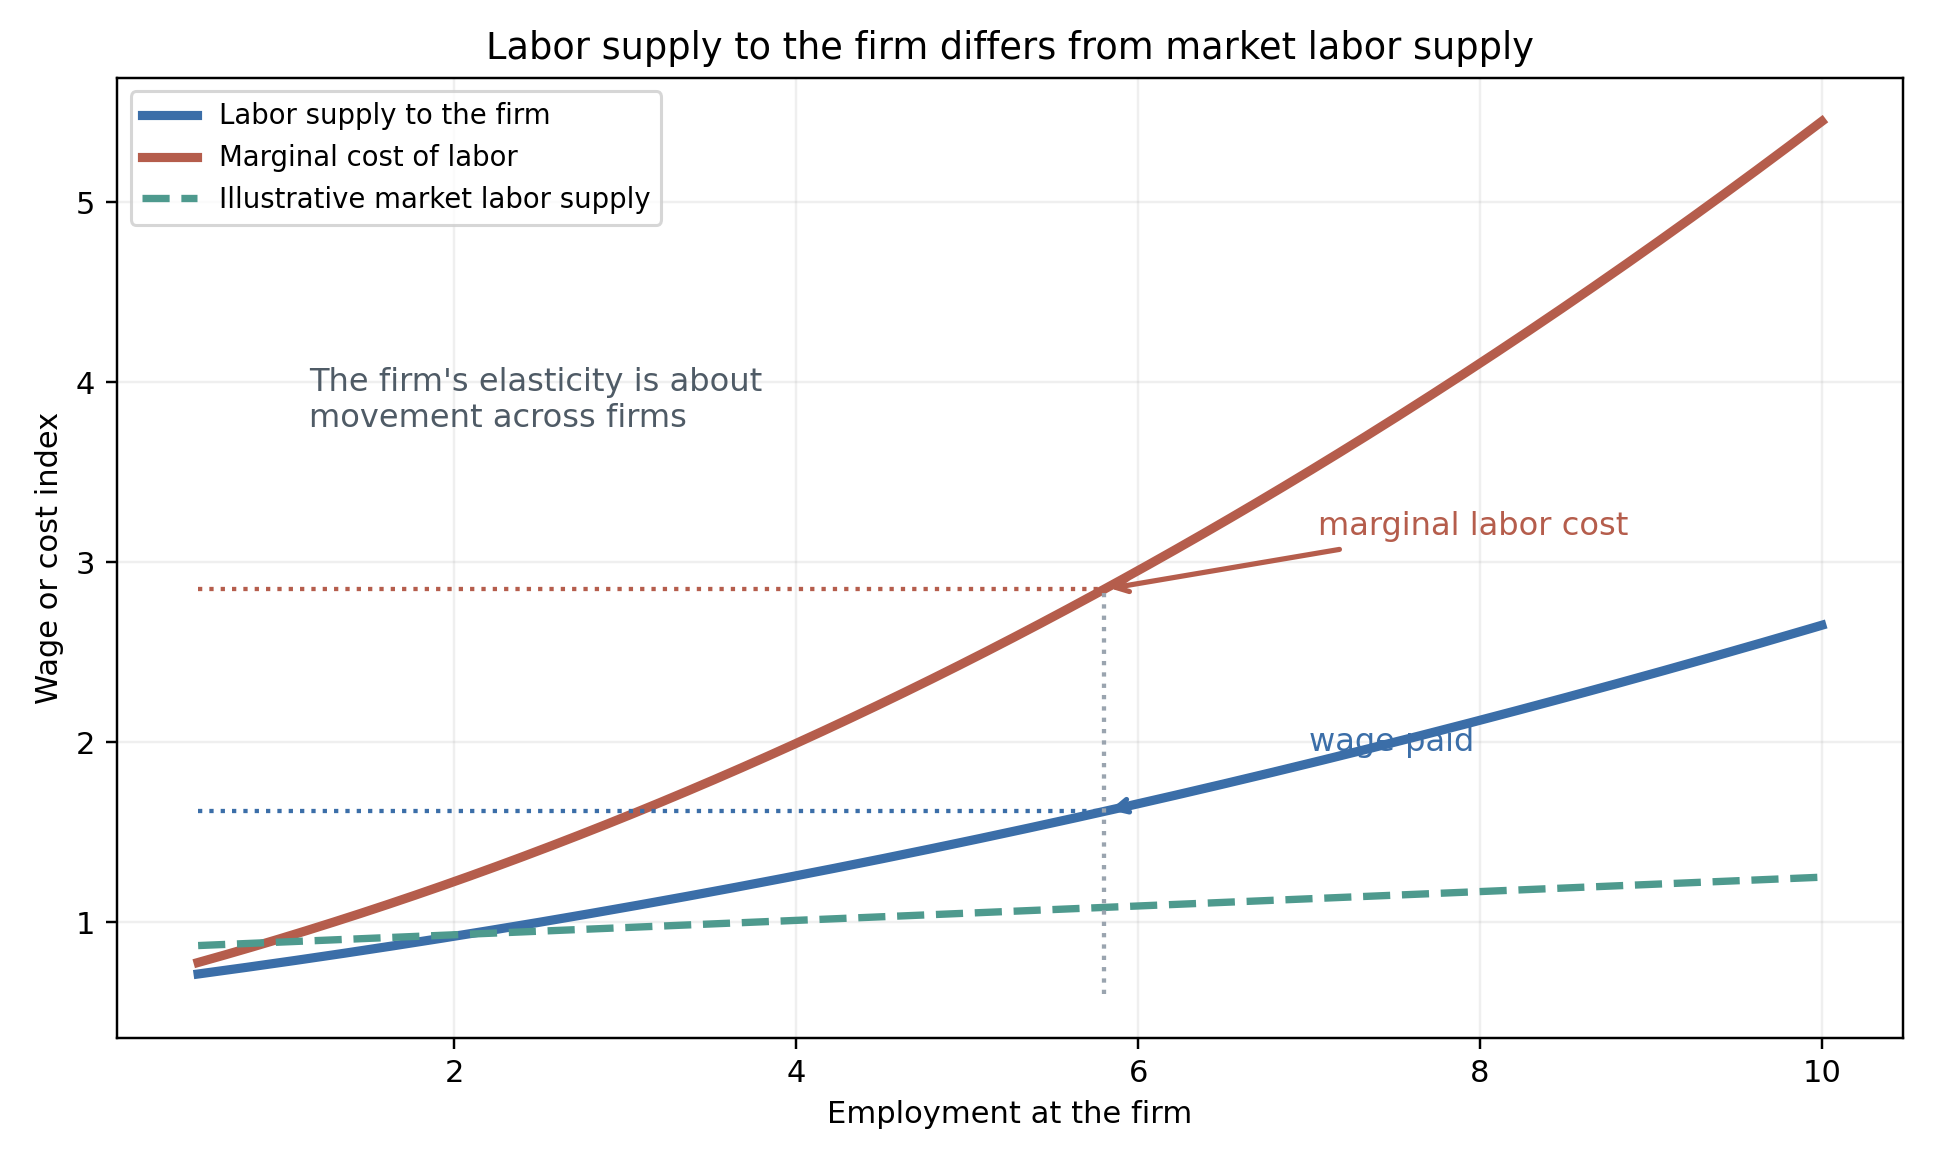
\includegraphics[height=0.72\textheight]{06-labor-supply-to-the-firm.png}
\end{center}
\end{frame}

\begin{frame}{Marginal labor cost and markdowns}
\[
MCL = w \left(1 + \frac{1}{\varepsilon_{N,w}}\right)
\qquad
\mu = \frac{MRPL}{w}
\]

\begin{itemize}
    \item Finite labor-supply elasticity means the marginal cost of labor exceeds the wage.
    \item A markdown summarizes the wedge between marginal revenue product and pay.
    \item Markdowns, firm wage premia, and rent-sharing are related but non-identical objects.
\end{itemize}
\end{frame}

\begin{frame}{Concentration is not the same thing as monopsony}
\[
HHI_m = \sum_j s_{jm}^2
\]

\begin{itemize}
    \item Concentration is an observable proxy, not a structural wage-setting parameter.
    \item Market boundaries may be mismeasured relative to actual worker outside options.
    \item Amenities, information frictions, and mobility costs can generate power even with many firms.
\end{itemize}
\end{frame}

\begin{frame}{Measurement objects in the literature}
\small
\begin{tabular}{p{0.23\linewidth} p{0.2\linewidth} p{0.21\linewidth} p{0.24\linewidth}}
\toprule
Approach & Variation & Margin & Main latent object \\
\midrule
Applications / tasks & Wage changes & Recruiting elasticity & Off-platform outside options \\
Quit elasticity & Wage differences & Retention / quits & Unseen offer network \\
Markdowns & Production moments & MRPL-wage wedge & True MRPL and structure \\
Concentration & Market shares & Wage differences & Correct market boundary \\
Mergers & Consolidation shock & Wage response & Deeper structural wedge \\
Firm shocks & Productivity or revenue & Pass-through & Sorting vs power \\
\bottomrule
\end{tabular}
\end{frame}

\begin{frame}{Empirical designs and what they identify}
\begin{itemize}
    \item Dube, Jacobs, Naidu, and Suri: direct wage variation, task-level unit, applications or fill margin, labor-supply elasticity to the firm.
    \item Yeh, Macaluso, and Hershbein: plant or firm unit, production-side moments, markdown object, stronger structural assumptions.
    \item Prager and Schmitt: merger shock, market structure changes, wage response to consolidation, partial view of labor market power.
\end{itemize}
\end{frame}

\begin{frame}{Measurement map}
\begin{center}
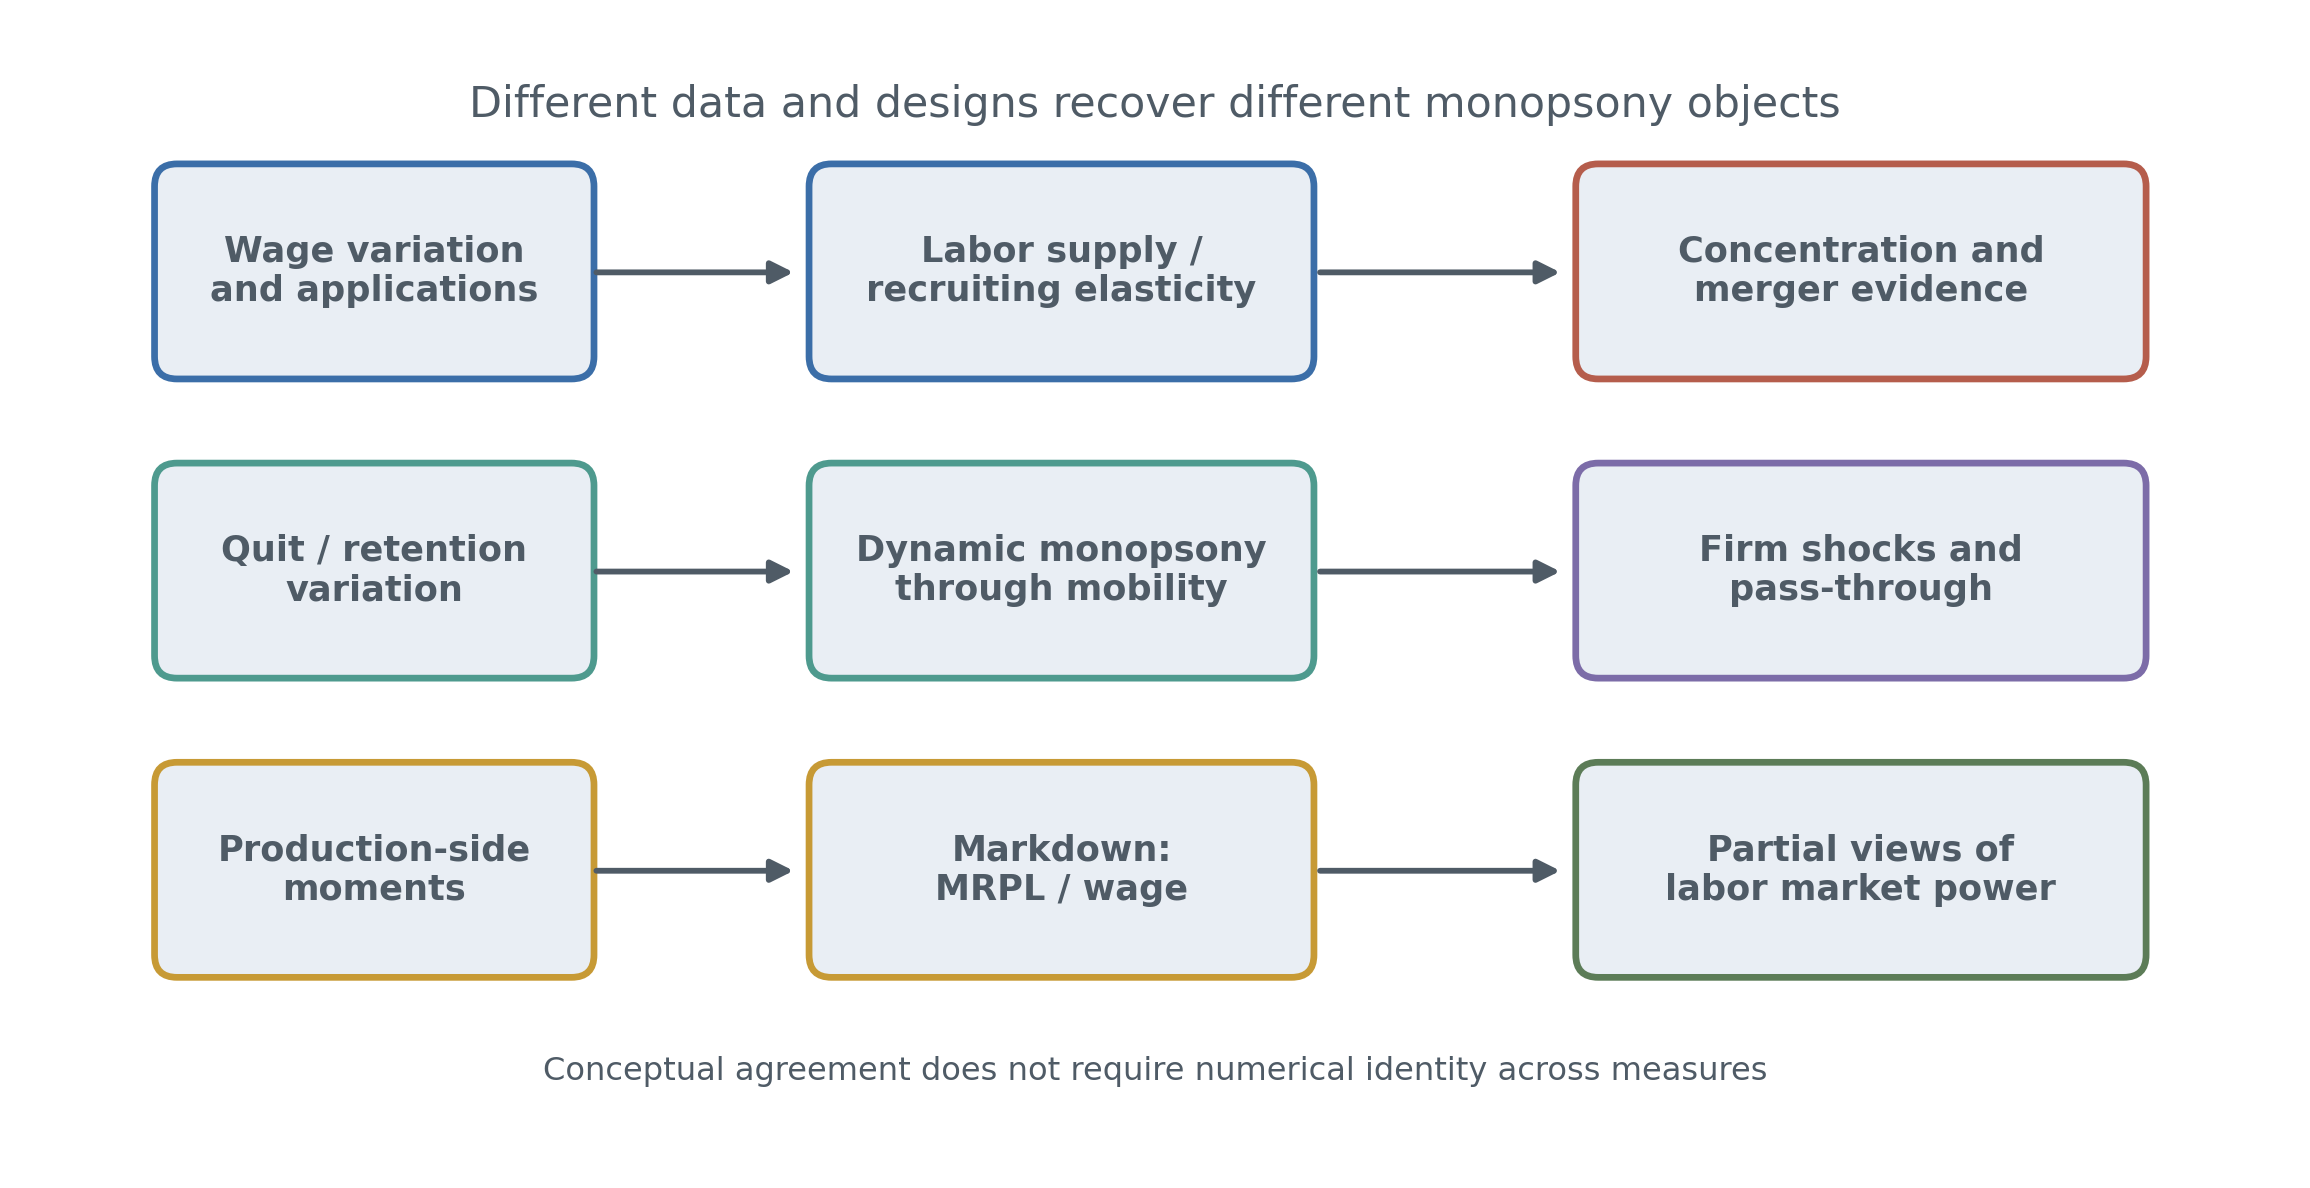
\includegraphics[height=0.72\textheight]{06-markdown-measurement-map.png}
\end{center}
\end{frame}

\begin{frame}{Sources of monopsony power}
\begin{itemize}
    \item Search and mobility frictions.
    \item Amenities and job differentiation.
    \item Information frictions and wage opacity.
    \item Geographic and occupational thinness.
    \item Concentration, large employers, and mergers.
    \item Contracts, licensing, visas, and internal wage rules.
\end{itemize}
\end{frame}

\begin{frame}{Sources map}
\begin{center}
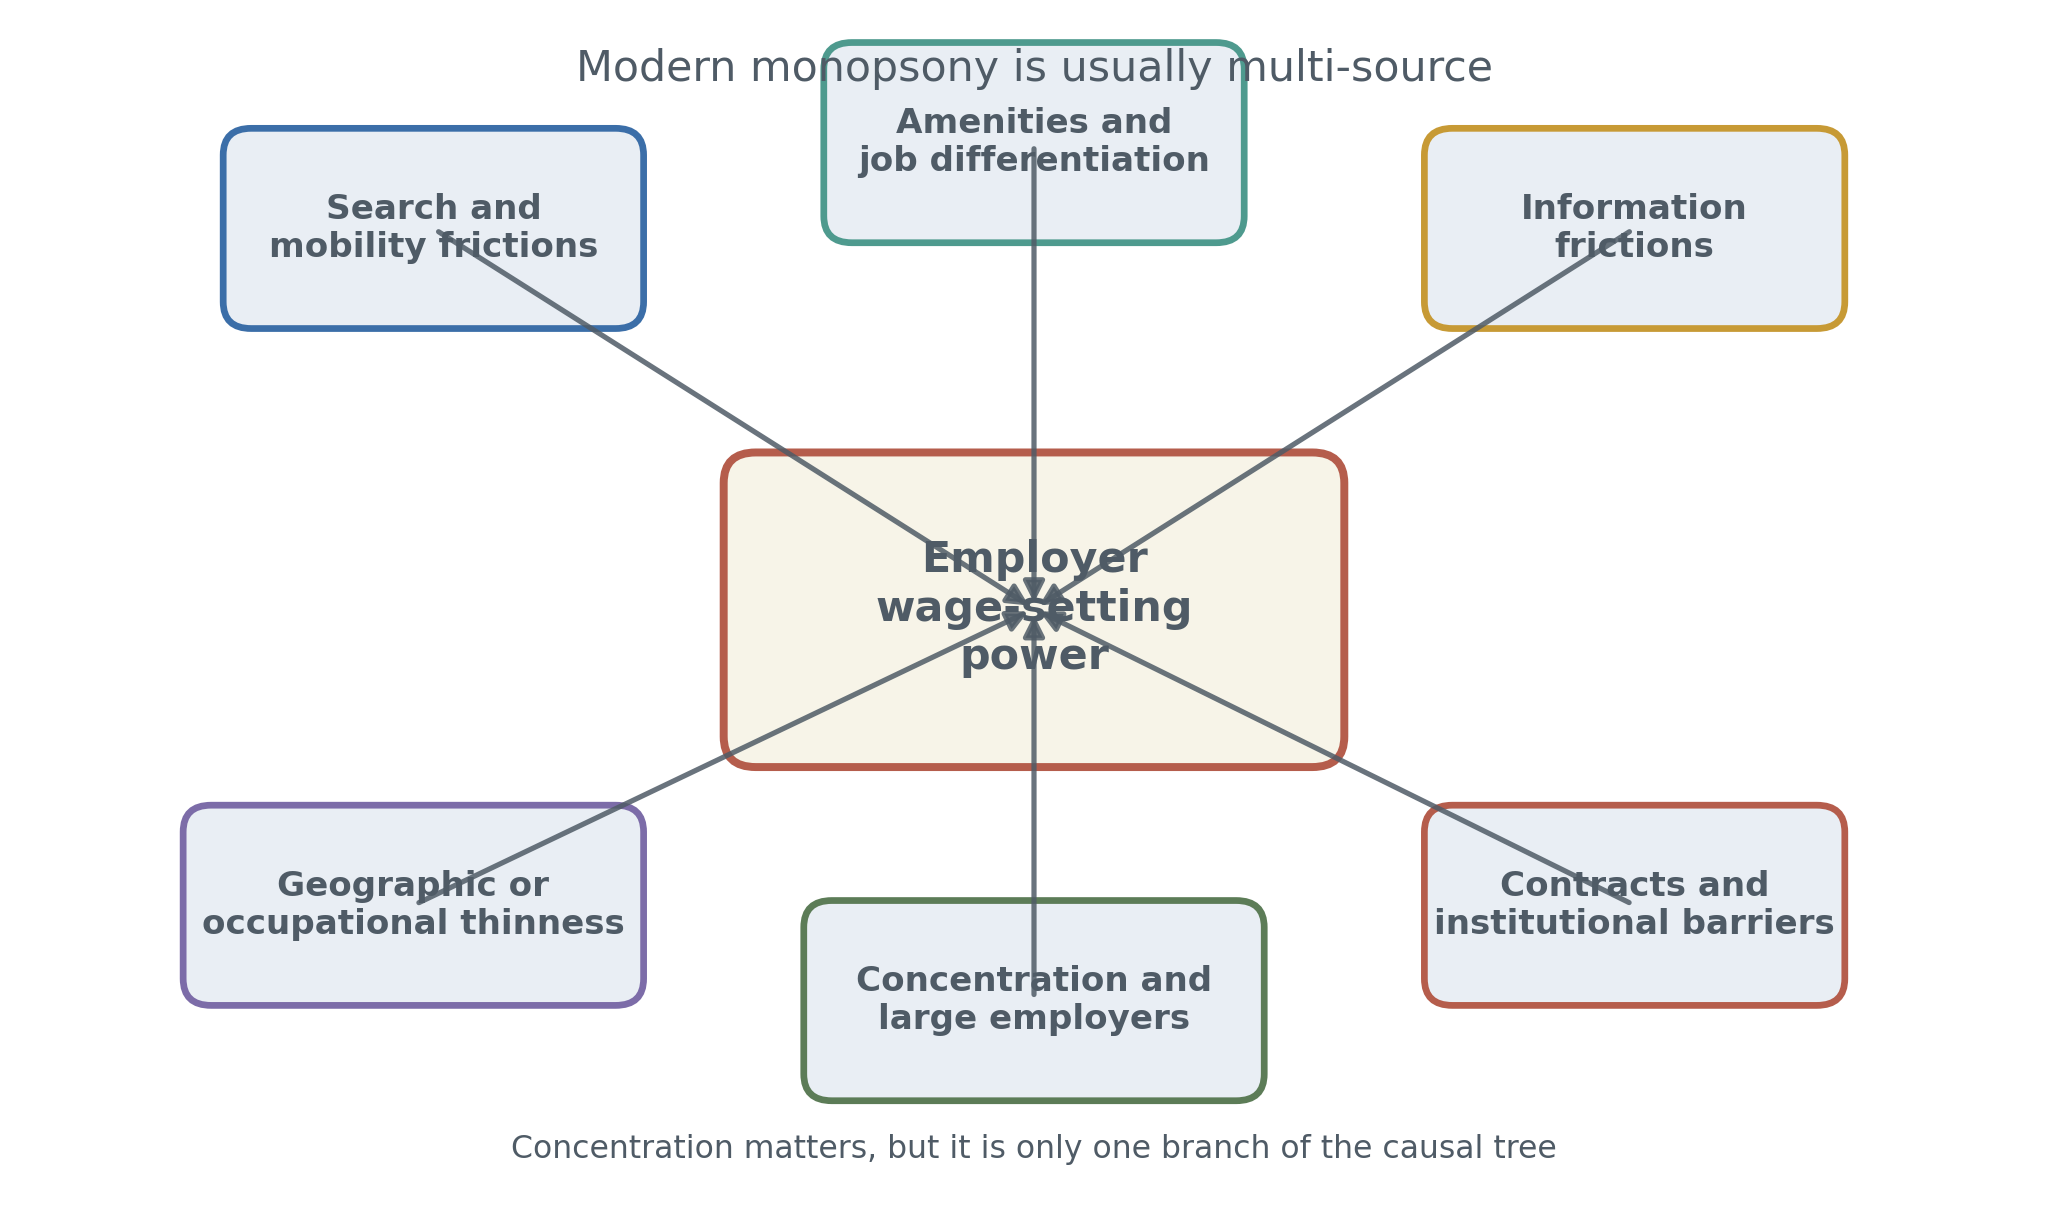
\includegraphics[height=0.72\textheight]{06-sources-of-monopsony-power.png}
\end{center}
\end{frame}

\begin{frame}{Frontier extension block}
\begin{itemize}
    \item Why concentration can understate or misclassify true power.
    \item Markdown measurement outside manufacturing and production settings.
    \item Amenities, compensating differentials, and worker beliefs.
    \item New data: vacancies, platforms, worker-firm panels, and mobility networks.
    \item Open link: monopsony, inequality, sorting, and policy design.
\end{itemize}
\end{frame}

\begin{frame}{Bridge to Week 7}
\begin{itemize}
    \item If firms have wage-setting power, minimum wages do not map into the competitive benchmark.
    \item The policy block becomes about incidence under imperfect competition.
    \item Week 7 starts with wage floors and asks how employer power changes predicted employment and wage effects.
\end{itemize}
\end{frame}

\begin{frame}{Takeaways}
\begin{itemize}
    \item Monopsony is best treated as a spectrum of employer wage-setting power.
    \item Labor supply to the firm is the core object; market concentration is only one possible proxy.
    \item Different empirical designs identify different wedges, so the measures need not coincide numerically.
    \item Modern monopsony usually comes from multiple overlapping sources, not a single mechanism.
\end{itemize}
\end{frame}

\appendix

\begin{frame}{Appendix: lab bridge}
\begin{itemize}
    \item Reproduce: Dube-style online labor elasticity from direct wage variation.
    \item Diagnose: Yeh-style markdown object from a synthetic plant panel.
    \item Transfer: Prager-Schmitt-style merger or concentration panel.
    \item Keep the object, variation, observed margin, and latent object separate in every exercise.
\end{itemize}
\end{frame}

\end{document}
